\chapter{Conclusions and Future work}
\section{Conclusions}
This thesis effectively connects \acrshort{cl} and traditional \acrshort{dl} methods for classifying glitches in \acrshort{gw} data. By combining strain data with auxiliary channel data using a multimodal fusion framework, the research shows notable enhancements in classification accuracy and provides a more profound understanding of glitch properties. The study emphasizes several important discoveries: 
\begin{itemize}
    \item \textbf{Effectiveness of \acrshort{cl} strategies}: The implementation of various \acrshort{cl} strategies such as Naive \acrshort{cl}, \acrfull{lwf}, \acrfull{agem}, \acrfull{ewc}, \acrfull{der}, DER++, and \acrfull{scr} revealed that while the Naive approach exhibited best performance, other methods also showed promise. \acrshort{agem} suffered from extreme catastrophic forgetting, indicating potential implementation issues or suboptimal hyperparameter choices. 
    \item \textbf{Multimodal Fusion}: Integrating strain data (Qscans) with auxiliary channel data (fractal dimension matrices) resulted in exceptional outcomes, reaching up to 100\% accuracy on the test set. This combination offered a more holistic view of the system, encapsulating various facets of the underlying physical processes and allowing the model to identify distinctive features not visible in individual modalities. 
    \item \textbf{The Avalanche Framework}: Although the Avalanche Framework was useful for managing multiple datastreams, it faced difficulties in smoothly integrating diverse modalities and computing \acrshort{cl}-specific metrics. Future research should explore alternative frameworks like Continuum and Sequoia for improved support and efficiency in multimodal environments. 
    \item \textbf{Research Methodology}: The research approach, based on thorough experimentation and analysis, confirmed the efficacy of multimodal fusion in classifying glitches. Employing convolutional networks with dropout and batch normalization layers was successful in distinguishing between glitch types, even with the limited auxiliary data available. 
\end{itemize}

\section{Future work}
The research done as described in \ref{sec-Research} and \ref{chap:models_and_results} is promising about the potential of investigating multi-modal fusion architectures for \acrshort{gw} analysis, the combination of Spectrogram Image Analysis combined with Fractal Dimensions of Auxiliary Channels gave outstanding results \ref{subsub:rq3}. \\
Further research, especially the integration of attention \citep{vaswani2017attention, niu2021review} should be investigated on additional fractal dimension data, preferably with more than 3 glitch categories. \\
Another topic of interest and research is how to succesfully apply \acrshort{cl} in a Multimodal setting. There is some research ongoing, one of the most notable solutions is the Climb benchmark \citep{srinivasan2022climb}. This benchmark is designed to study \acrshort{cl} for multimodal tasks where it evaluates models in two phases. An upstream phase where the model is trained on a sequence of tasks and evaluated on its ability to retain knowledge from previous tasks while learning new ones. And a downstream phase where the model is evaluated on the ability to transfer knowledge to new tasks with minimal data.\\
The application of Multimodal Machine Learning (MMML) has already been succesfully applied in other \acrshort{gw} signal studies. An example of such applications is found in \citep{cuoco2021multimodal}, where a Multimodal strategy is applied to characterize Gamma-Ray Bursts (GRB) from Binary Neutron Star Mergers. The two modalities the researchers apply are the strain gravitational wave signal and the GRB light curve, see Figure \ref{fig:multimodal_redshift} for a visualisation of the architecture. The calculated redshift can then be used to understand the distance and properties of astrophysical events. 

\begin{figure}[hb]
    \centering
    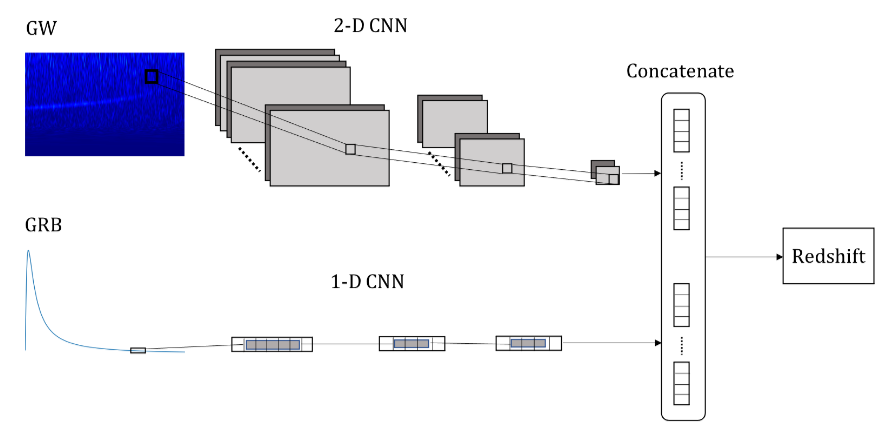
\includegraphics[width=0.8\textwidth]{Grad Assignment/Images/futureWork.png}
    \caption{Multimodal ML model to compute redshift of joint GW and GRB sources. \citep{cuoco2021multimodal}}
    \label{fig:multimodal_redshift}
\end{figure}
